\Chapter{Caudal Vein Plexus Feature Extraction}
The study of the zebrafish CVP and its utilization as a model for screening assay has not been as prevalent as the ISV, and very few studies have attempted to identify regulators of CVP development. Previous research has primarily focused on using color, texture \cite{Tran07} and morphological changes \cite{Feng05} for toxicity analysis. Shape information, however, can be another attribute that can be evaluated. A shape descriptor can capture the outline of the shape that other color or texture-based descriptors may not be able to capture. Hence
by quantification of the shape of CVP, and comparing it against that of a healthy embryo, we can identify changes in CVP due to exposure to toxins. This chapter will discuss utilization of histogram of oriented gradients (HOG), co-occurrence of histogram of oriented gradients gradient (Co-HOG) and weighted co-occurrence histogram of oriented gradients (gCo-HOG) for shape modeling.

\section{Histogram of Oriented Gradients}

HOG descriptor first proposed by Dalal and Triggs \cite{Dalal05} has been used in many different problems in computer vision, such as pedestrian detection \cite{Wada09}, face recognition \cite{Deniz11}, object recognition \cite{Bosch07} and text recognition \cite{Wang10}. HOG features are extracted from image by first computing gradient orientation at every pixel. Orientations of gradients are quantized into histogram bins and each bin has an orientation range. Image is divided into blocks and in each block a histogram of oriented gradients is computed. HOG feature consists of concatenation of histogram of oriented gradients over all blocks. 
\begin{figure}[htb] 
 \centering
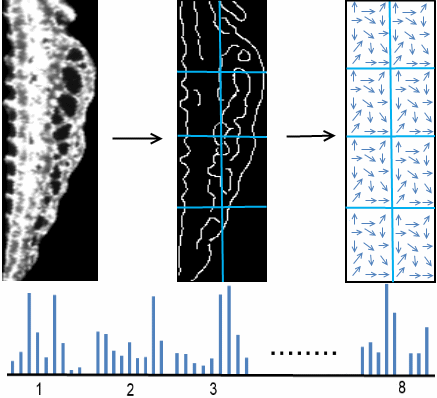
\includegraphics[scale=0.3]{figure/hog.png}
  \caption{ Extraction of HOG features from a CV image. (left) Original image. (center) Edge contours are extracted using an edge detector, image is divided into 8 blocks. (right) HOG vector is extracted from each sub region. (bottom) Concatenation of all the HOG vectors to obtain the HOG features for image.}
 \label{hog}
\end{figure}
In our case, HOG are computed on edge contours extracted using the canny edge detector (fig \ref{hog}). The HOG descriptor is quantized into $K$ orientation bins, each over an orientation range. The weight from each contour point depends on its gradient magnitude and is added to its orientation bin. Each bin in the histogram represents the sum of gradient magnitudes that have orientations within a certain angular range. The HOG is normalized to sum to unity. To compare the effect of orientations, we generate histograms with orientation range from $[0, 360]$ and $[0, 180]$. Histograms with $K$ ranging from 6 to 20 are evaluated. 

HOG are invariant to 2d rotation and illumination variations. On the other hand, HOG captures orientation of only isolated pixels, ignoring spatial relationship among neighboring pixels. Co-HOG captures spatial information and is more powerful in describing local structure. With spatial structure, more shape information of object can be captured.

\subsection{Co-occurrence of Histogram of Oriented Gradients}
Co-HOG is an extension of HOG. Co-HOG captures spatial information by measuring probability of oriented gradients between pairs of pixel. A pixel pair can be represented by an offset $(x, y)$, which captures the spatial relationship of the two points. As shown in fig \ref{cohog}(left), we define 31 offsets including zero offset for a given point. The black pixel in the center is the pixel under consideration and the neighboring blue pixels are with different offsets. Each neighboring pixel in blue color forms an orientation pair with the center black pixel and accordingly votes to the co-occurrence matrix. For each pixel in the image of size $M \times N$, the orientations ranging between $[0, 360]$ are quantized into eight orientation bins. Co-occurrence matrix at a specific offset $(x, y)$ is defined as:
			\small
			\begin{equation}\label{eq:cohog}
				C_{x,y}(i, j) = \sum_{p}\sum_{q}\begin{cases} 1, & \mbox{if } I(p, q) = i, I(p + x, q + y) = j\\ 
				0, &  otherwise \end{cases} 
				\end{equation} 
				\normalsize 
Co-HOG obtains 31 co-occurrence matrices. There are $8 \times 8 = 64$ elements in the co-occurrence matrix (fig \ref{cohog}(right)). The co-occurrence matrix calculated with zero offset has only 8 values. 8 rectangular regions are tiled $M/4 \times N/2$ with no overlap. More tiles are made along the image width as CV occupies more region along width as compared to height. Finally, co-occurrence matrices from all the rectangular regions are concatenated into one vector. Thus the dimension of our feature is $(64 \times 30 + 8) \times 8 = 15424$. Co-HOG extracts both local and global shape information, with varying offset sizes. 

One potential limitation of co-occurrence histograms of oriented gradients is that both strong and weak gradients provide the same contribution in representing the spatial structure.  To address this limitation, we investigate the inclusion of gradient strength in the generation of the histogram.
\begin{figure}[htb] 
 \centering
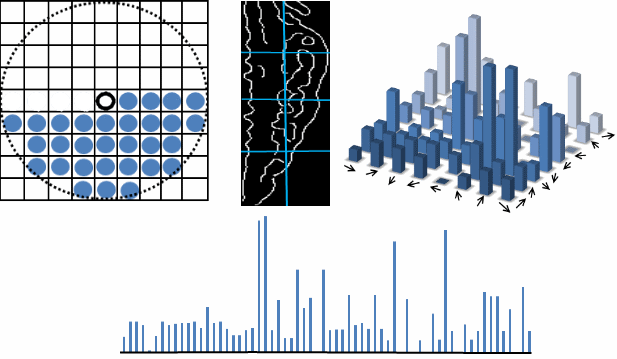
\includegraphics[scale=0.35]{figure/cohog.png}
  \caption{ Extraction of Co-HOG features from a CV image. (left) Pixel offset. (center) Edge contours are extracted using an edge detector, image is divided into 8 blocks. (right) Co-HOG vector is extracted from one region. (bottom) concatenation of all the Co-HOG vectors to obtain the Co-HOG features for image.}
 \label{cohog}
\end{figure}
As shown in \cite{Pang12}, we treat gradient as forces and use vector addition to combine forces using:
				\small
				\begin{equation}\label{eq:add}
				C_{x,y} = C_{x,y} + \|g_{1} + g_{2}\| 
				\end{equation}
				\normalsize 
where $C$ is the co-occurrence matrix at a specific offset $(x, y)$ as defined in Equation \ref{eq:cohog}, $g_{1}$ is the gradient magnitude at location $(p, q)$, and $g_{2}$ is the gradient magnitude at location $(p + x, q + y)$. The gCo-HOG feature descriptor of the whole image can then be constructed by concatenating all the regions features. The gCo-HOG is normalized to sum to unity.
